\chapter{Intelligent Ride Matching and Predictive System}

\section{Introduction}

The previous chapter established a complete ride management system with real-time synchronization capabilities. However, its behavior remained primarily reactive: users had to explicitly initiate actions such as searching for rides or offering trips, and the platform responded based on predefined rules.

This chapter introduces an additional decision layer aimed at making the system more adaptive and proactive. The goal is not only to react to user requests, but also to improve how the platform identifies opportunities and anticipates user needs.

Two complementary approaches are developed:

\begin{itemize}
    \item \textbf{Sprint 4 — Smart Matching System}: an algorithmic layer that enables dynamic ride matching based on route overlap and optimized pickup points.
    \item \textbf{Sprint 5 — Machine Learning System}: a predictive layer that models user behavior to anticipate ride needs and provide proactive suggestions.
\end{itemize}

Together, these components extend the platform beyond reactive behavior, improving ride utilization, reducing missed opportunities, and enhancing overall interaction efficiency.

% =========================================================
\section{Problem Definition}

Most traditional ride-sharing systems rely on strict origin-destination matching~\cite{furuhata2013ridesharing}. A ride is suggested only when the passenger’s request closely matches the driver’s route.

This limitation leads to missed opportunities. In many real scenarios, routes partially overlap without sharing identical starting points.

For instance, consider a driver traveling from point A to point C, and a passenger requesting a ride from point B to point C. Even though the passenger lies along the driver’s path, conventional systems often fail to detect this match due to rigid constraints.

Another limitation concerns user interaction. The system depends entirely on manual actions, requiring users to repeatedly search for rides. This becomes inefficient in cases where behavior follows recurring patterns, such as daily commuting.

To address these issues, this chapter introduces two complementary solutions:

\begin{itemize}
    \item \textbf{Route-based intelligent matching}, enabling detection of spatial overlap and dynamic ride insertion.
    \item \textbf{Behavior prediction}, enabling proactive ride suggestions based on learned user patterns.
\end{itemize}

% =========================================================
\section{Sprint 4: Smart Matching System}

\subsection{Overview}

The Smart Matching System introduces a trajectory-based approach to ride matching~\cite{stiglic2015flexible}.

Instead of treating rides as simple origin-destination pairs, each ride is modeled as a continuous path. This allows the platform to identify intermediate opportunities where passengers can join an existing route.

The shift from point-based to route-based matching significantly increases the number of viable matches, while still preserving route coherence for drivers.

% ------------------------
\subsection{Sprint Backlog}

The objective of this sprint is to design and implement a route-based matching system capable of identifying ride opportunities through spatial trajectory analysis and optimizing pickup interactions.

The backlog can be grouped into three main categories:

\begin{itemize}
    \item \textbf{Spatial Modeling}: trajectory representation and corridor construction,
    \item \textbf{Matching Logic}: filtering, scoring, and optimization,
    \item \textbf{System Integration}: lifecycle adaptation and notification handling.
\end{itemize}
\begin{table}[H]
\centering
\renewcommand{\arraystretch}{1.4}
\setlength{\tabcolsep}{6pt}
\begin{tabular}{|p{10cm}|c|}
\hline
\textbf{User Story} & \textbf{Priority} \\
\hline
As a user, I want to find rides even if my pickup point is not exactly the driver's origin so that more ride opportunities are available & High \\
\hline
As a driver, I want to accept passengers along my route without significant detours so that my experience remains convenient & High \\
\hline
As a system, I want to represent rides as continuous trajectories to enable spatial matching & High \\
\hline
As a system, I want to construct a spatial corridor around each route to detect nearby passenger requests & High \\
\hline
As a system, I want to filter candidate rides based on time constraints and seat availability & High \\
\hline
As a system, I want to compute optimal pickup points along the route to minimize detour and travel time & High \\
\hline
As a system, I want to evaluate and rank candidate matches using scoring criteria such as detour distance and feasibility & High \\
\hline
As a system, I want to adapt the ride lifecycle to support intermediate pickups & Medium \\
\hline
As a user, I want to receive notifications about relevant ride matches so that I can act immediately & High \\
\hline
As a system, I want to validate matching accuracy and ensure consistency across different scenarios & Medium \\
\hline
\end{tabular}
\caption{Sprint 4 Backlog — Smart Matching System}
\end{table}
The backlog reflects the progressive construction of the matching system, from spatial representation to filtering, scoring, and integration into the ride lifecycle.

The sprint was developed incrementally. Core components such as trajectory modeling and corridor filtering were implemented first to establish a solid foundation.

After validation, additional elements such as scoring and lifecycle adaptation were introduced, ensuring that each component was tested before integration into the complete matching pipeline.
\subsection{Problem Reframing}

The matching problem is reformulated from a discrete comparison task into a geometric optimization problem.

Instead of checking whether two rides share identical endpoints, the system evaluates whether a passenger’s location can be integrated into a driver’s trajectory under feasible conditions. This change reflects a more realistic view of how rides occur in practice, where routes often overlap partially rather than exactly.

This reformulation introduces two main challenges:

\begin{itemize}
    \item efficient detection of spatial proximity between trajectories,
    \item identification of a pickup point that minimizes disruption to the existing route.
\end{itemize}

A key difficulty lies in balancing flexibility and feasibility. While increasing the search space allows more potential matches, it also introduces the risk of proposing solutions that are impractical in real-world conditions.

It is important to note that the proposed approach does not rely on simple point-to-point distance comparisons. Such methods ignore the structure of the road network and do not reflect actual travel feasibility.

Instead, candidate rides are evaluated through a multi-stage scoring process~\cite{routing}. The passenger’s location is projected onto the driver’s trajectory, detour cost is estimated, and candidates are ranked using both spatial and temporal criteria. This guarantees that matching decisions remain grounded in realistic travel constraints.

The reformulation shifts the problem from a basic geometric comparison to a constrained route-insertion problem, where the objective is to identify a feasible pickup location that preserves route continuity while minimizing additional cost.

Alternative strategies, such as nearest-point matching or grid-based partitioning, were considered. However, these approaches either ignore route structure or introduce excessive approximation. The corridor-based method offers a more balanced solution in terms of flexibility, accuracy, and computational cost, while remaining compatible with real-time constraints.
% ------------------------
\subsection{Route-Based Matching Concept}

Each ride is modeled as a geometric trajectory rather than a fixed pair of points. Passenger requests are evaluated against this trajectory.

A match is identified when the passenger’s pickup location falls within a spatial corridor defined around the driver’s route~\cite{chen2011trajectory}. This allows the platform to detect opportunities that would otherwise be missed under strict origin-destination matching.

\begin{figure}[H]
\centering
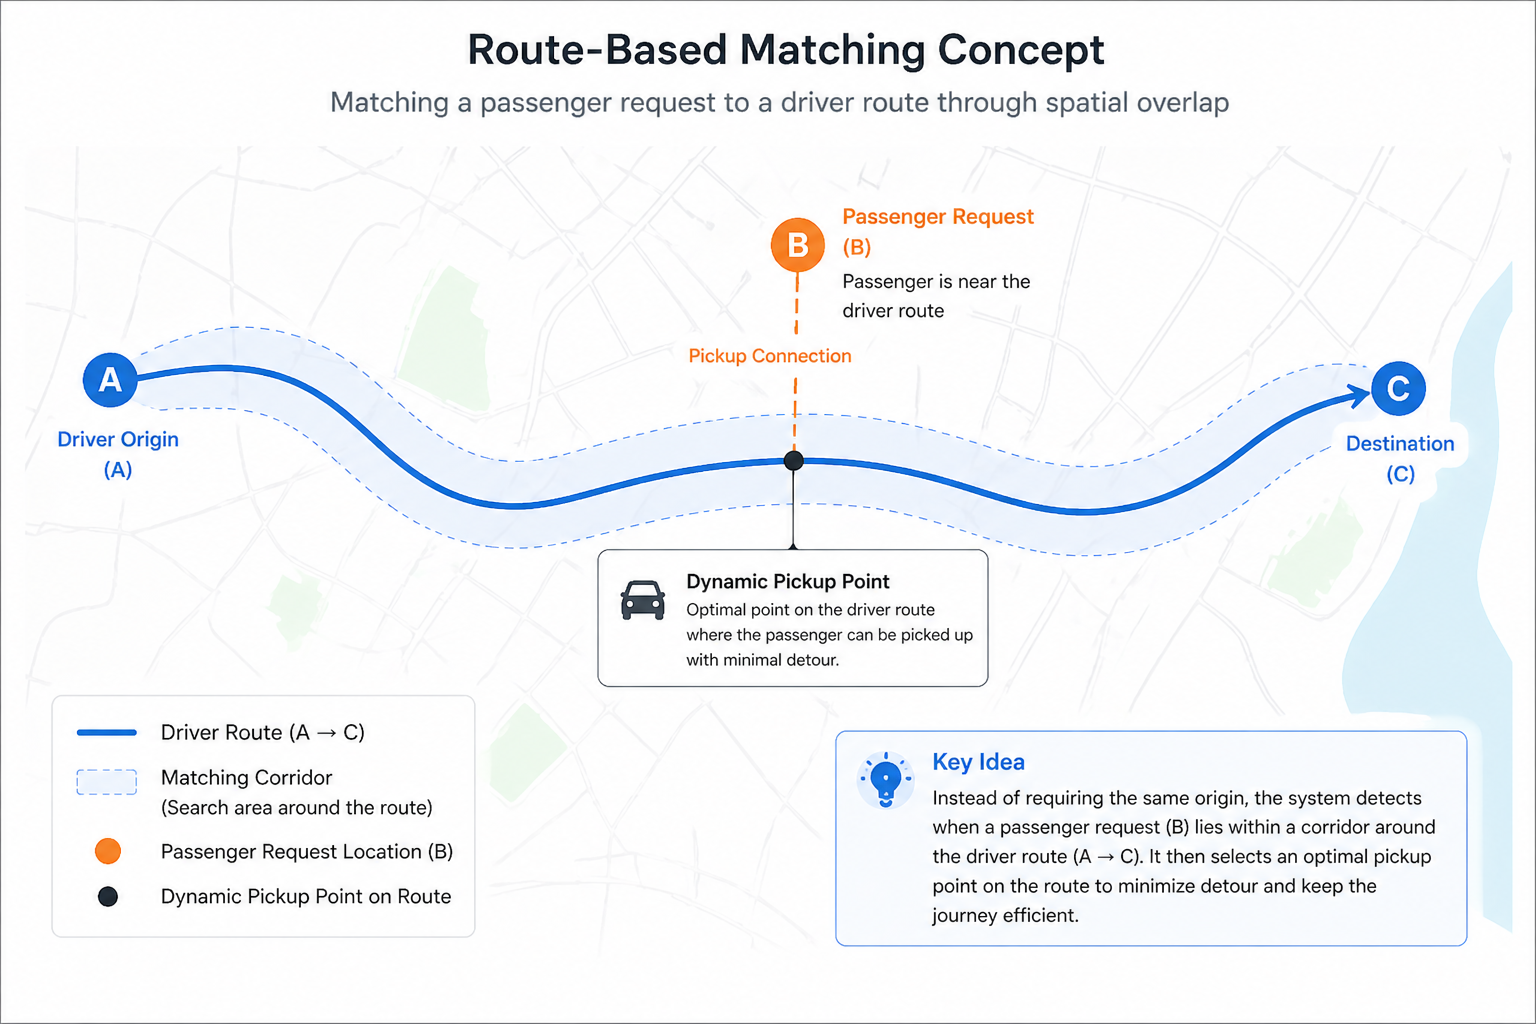
\includegraphics[width=0.9\textwidth]{images/architecture/route_matching.png}
\caption{Route-Based Matching Concept}
\end{figure}

% ------------------------
\subsection{Matching Pipeline}

The matching process is organized as a multi-stage pipeline that progressively reduces the number of candidate rides:

\begin{itemize}
    \item \textbf{Validation}: filters rides based on temporal compatibility, seat availability, and ride status.
    
    \item \textbf{Route Analysis}: represents rides as continuous trajectories using polyline encoding.
    
    \item \textbf{Corridor Filtering}: retains only candidates located within a spatial corridor around the driver’s route, reducing the search space.
    
    \item \textbf{Scoring}: ranks candidates according to detour distance, additional travel time, and pickup feasibility.
\end{itemize}

The staged structure limits unnecessary computations and focuses processing on relevant candidates, improving both efficiency and matching quality.

\begin{figure}[H]
\centering
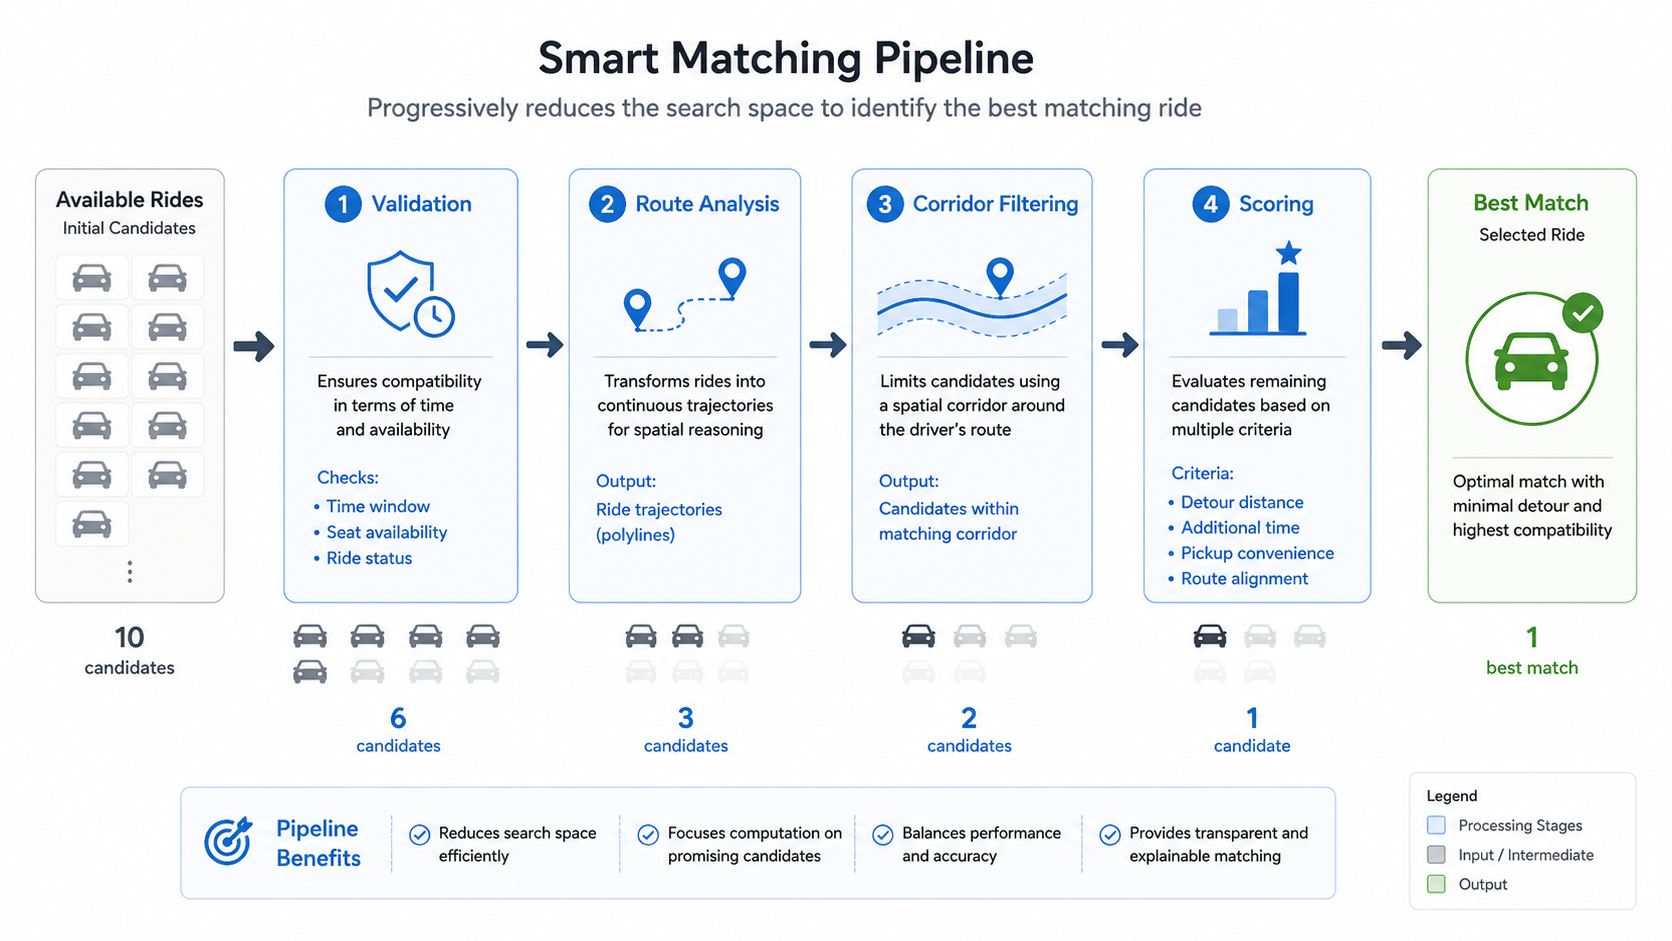
\includegraphics[width=0.95\textwidth]{images/architecture/matching_pipeline.png}
\caption{Smart Matching Pipeline}
\end{figure}

% ------------------------
\subsection{Matching Score Formalization}

Each candidate is assigned a composite score based on four weighted factors. Let $d_p$ denote the normalized distance between the passenger's origin and the driver's route, $d_d$ the normalized distance between the passenger's destination and the driver's destination, $\Delta t$ the temporal compatibility, and $s$ the normalized seat availability. The score $S$ is defined as:

\begin{equation}
S = 0.40 \, d_p + 0.30 \, d_d + 0.20 \, \Delta t + 0.10 \, s
\end{equation}

Only candidates satisfying $S \geq \tau$, where $\tau$ is a predefined threshold, are returned to the user.

% ------------------------
\subsection{Dynamic Pickup Optimization}

Unlike traditional systems where pickup points are fixed, the proposed approach determines a suitable pickup location dynamically.

The selected point aims to minimize detour distance while remaining accessible to both driver and passenger. This optimization takes into account route continuity and geographic constraints.

A key design choice is the prioritization of driver convenience. Since drivers are not financially incentivized, limiting additional effort is essential for maintaining participation.

To support decision-making, the system computes and presents the detour cost associated with each match, allowing users to evaluate trade-offs before confirming a ride.

% ------------------------
\subsection{Ride Lifecycle Adaptation}

The matching process is tightly integrated into the ride lifecycle.

Rather than treating matching as a static pre-processing step, the proposed approach dynamically adapts the execution flow. A ride initially defined as A → C can evolve into a multi-stage process:

\begin{itemize}
    \item Initial departure from A
    \item Intermediate pickup at B
    \item Continuation to C
\end{itemize}

Such transformation reflects the dynamic nature of real-world ride-sharing, where new participants can be incorporated during execution without redefining the entire trip.

From a system perspective, this requires the lifecycle model to support intermediate states and transitions. The ride is no longer a fixed sequence, but a flexible structure that can accommodate additional events such as pickups or minor route adjustments while maintaining consistency.

The integration ensures that matching is not an isolated computation, but directly influences platform behavior and execution consistency. Each accepted match triggers updates in ride state, participant roles, and route progression, ensuring that all components remain synchronized.

As a result, the lifecycle becomes an active component of the matching system, enabling seamless coordination between planning and execution phases.
\subsection{Intelligent Notification System}

To ensure that detected matches lead to effective user actions, the platform incorporates a notification mechanism that connects backend computation with user interaction.

Unlike conventional notification systems that simply report events, this approach delivers contextual and actionable information. Notifications are triggered only when a relevant matching opportunity is identified and include details such as pickup feasibility, detour impact, and route alignment.

This selective strategy prevents unnecessary alerts while ensuring that users are informed of meaningful opportunities.

The interaction flow is illustrated below.

\begin{figure}[H]
\centering
\begin{minipage}[t]{0.43\textwidth}
    \centering
    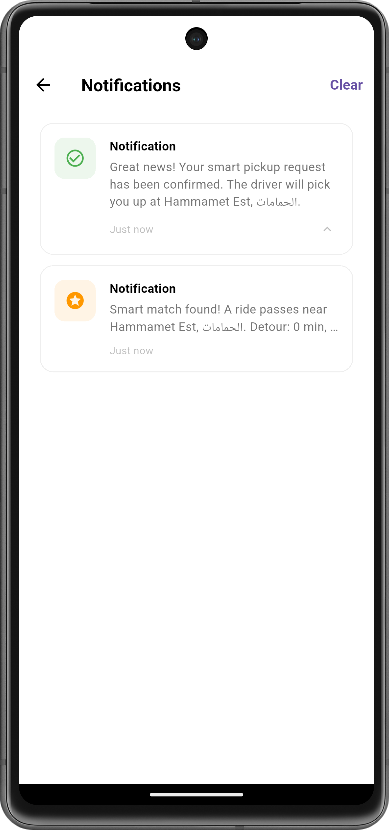
\includegraphics[width=\textwidth]{images/ui/smart_notification_preview.png}
    \caption*{(a) Smart Notification Preview}
\end{minipage}
\hfill
\begin{minipage}[t]{0.43\textwidth}
    \centering
    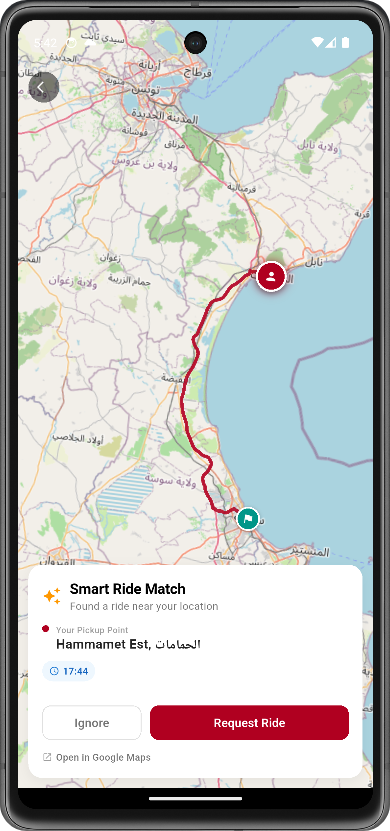
\includegraphics[width=\textwidth]{images/ui/smart_match_screen.png}
    \caption*{(b) Smart Match Screen}
\end{minipage}
\caption{Intelligent Notification Flow}
\end{figure}

The notification first appears as a concise preview, allowing the user to quickly assess its relevance. Upon interaction, the user is redirected to a dedicated interface presenting detailed information about the proposed match.

Matching results are therefore not passively displayed, but actively integrated into the user workflow through a transition from notification to decision.

The mechanism ensures that the matching engine is not only computationally effective but also operationally meaningful, transforming detected opportunities into actionable user interactions.
% ------------------------
\subsection{Sprint Validation and Testing}

The Smart Matching System was validated through scenario-based evaluation focusing on both correctness and system impact.

\begin{itemize}
    \item \textbf{Matching Accuracy}: verification that valid spatial overlaps are correctly detected.
    
    \item \textbf{Filtering Efficiency}: confirmation that irrelevant candidates are eliminated early in the pipeline.
    
    \item \textbf{Detour Computation}: validation of distance and time calculations across different scenarios.
    
    \item \textbf{Lifecycle Consistency}: ensuring that ride state transitions remain coherent after match insertion.
\end{itemize}

Comparative scenarios were also analyzed:

\begin{itemize}
    \item strict origin-destination matching versus route-based matching,
    \item manual ride discovery versus system-assisted matching.
\end{itemize}

The results show that the proposed approach increases matching coverage while maintaining execution consistency and system stability.

% ------------------------
\subsection{System Impact}

The Smart Matching System introduces a significant improvement in ride discovery:

\begin{itemize}
    \item increases matching coverage beyond strict constraints,
    \item reduces missed ride opportunities,
    \item improves overall system utilization.
\end{itemize}

More importantly, it establishes a spatially-aware foundation for higher-level intelligent features.

\section{Sprint 5: Machine Learning System}

\subsection{Overview}

While the Smart Matching System improves the platform’s ability to respond to user requests, it still depends on explicit interaction. In practice, this introduces friction: users must repeatedly perform similar actions despite having consistent commuting habits.

The Machine Learning System addresses this limitation by introducing a predictive layer that anticipates user intent. Instead of waiting for a user to initiate a search, the proposed approach identifies recurring mobility patterns and surfaces relevant ride suggestions at appropriate moments.

The proposed layer shifts the platform from a purely reactive model toward a context-aware system that adapts progressively to user behavior.

From a system perspective, this component operates as an independent intelligence layer. It consumes historical trip data and produces probabilistic predictions that are integrated into the user interface without modifying the core ride lifecycle.

It is important to distinguish this component from the rule-based matching system introduced in the previous sprint. The Smart Matching System answers the question of \textit{who} can share a ride by evaluating spatial compatibility, whereas the Machine Learning System addresses \textit{when} a user is likely to need a ride, regardless of current availability.

These two mechanisms operate on complementary dimensions: matching remains reactive and deterministic, while prediction is proactive and probabilistic. The ML layer does not replace the matching logic; it operates upstream, suggesting potential needs that can later be handled through the existing workflow.

% ------------------------
\subsection{Problem Framing and Design Rationale}

The objective of this component is not generic prediction, but structured behavioral anticipation under constrained data conditions.

Unlike large-scale mobility platforms, this system operates in a controlled corporate environment characterized by:

\begin{itemize}
    \item limited historical data,
    \item a relatively small user base,
    \item highly repetitive commuting behavior.
\end{itemize}

These constraints directly influence the design choices.

Rather than relying on complex deep learning models, the system leverages the regularity of commuting patterns~\cite{liao2007learning}. Most users follow stable spatial and temporal routines, such as consistent origins, destinations, and departure times.

Based on this observation, the problem is decomposed into two complementary tasks:

\begin{itemize}
    \item identifying recurring patterns in user behavior,
    \item predicting whether a given pattern will occur at a specific time.
\end{itemize}

The separation leads to a modular pipeline where pattern detection and prediction are handled independently, improving both interpretability and maintainability.

% ------------------------
\subsection{Sprint Backlog}

\begin{table}[!htbp]
\centering
\renewcommand{\arraystretch}{1.4}
\setlength{\tabcolsep}{6pt}
\begin{tabular}{|p{10cm}|c|}
\hline
\textbf{User Story} & \textbf{Priority} \\
\hline
As a user, I want the system to learn my commuting habits so that I do not need to repeatedly search for the same rides & High \\
\hline
As a user, I want the system to suggest rides automatically at relevant times & High \\
\hline
As a system, I need to generate realistic synthetic data to simulate commuting behavior & High \\
\hline
As a system, I want to cluster geographic locations into zones to simplify spatial representation & High \\
\hline
As a system, I want to extract temporal and spatial features to model user behavior & High \\
\hline
As a system, I want to validate detected patterns to eliminate noise and irrelevant behavior & Medium \\
\hline
As a system, I want to predict the probability of future ride requests & High \\
\hline
As a system, I want to apply a threshold to ensure only relevant suggestions are displayed & Medium \\
\hline
As a user, I want to see proactive ride suggestions directly in the interface & High \\
\hline
As a system, I want to validate the accuracy and stability of predictions & Medium \\
\hline
\end{tabular}
\caption{Sprint 5 Backlog — Machine Learning System}
\end{table}

The backlog summarizes the main stages required to build the predictive system, from data preparation to user-facing integration.

It begins with synthetic data generation and spatial abstraction, followed by feature extraction and pattern validation. These steps establish the foundation for predictive modeling.

Subsequent tasks focus on estimating the probability of future ride requests and filtering results to ensure relevance before presenting suggestions to the user.

% ------------------------
\subsection{Data Strategy and Justification}

A key constraint of this project is the lack of sufficient real-world historical data.

To address this limitation, a synthetic dataset was generated to approximate realistic commuting behavior. Although synthetic data is often viewed as a compromise in machine learning workflows, its use in this context is both justified and appropriate.

This justification stems from the nature of the problem:

\begin{itemize}
    \item The feature space is low-dimensional, primarily defined by time, location, and frequency.
    \item The target behavior, namely commuting, exhibits strong regularity.
    \item Noise levels remain limited compared to open-ended prediction domains.
\end{itemize}

In contrast to domains such as image recognition or natural language processing, where data complexity is high and difficult to approximate, commuting behavior can be modeled using controlled distributions that capture recurring patterns~\cite{mitchell1997machine}.

The synthetic dataset was therefore designed to reproduce three fundamental characteristics:

\begin{itemize}
    \item \textbf{Temporal regularity}: repeated departures within consistent time intervals.
    \item \textbf{Spatial consistency}: clustering of origins and destinations around typical zones.
    \item \textbf{Behavioral repetition}: recurring trips observed over multiple days.
\end{itemize}

Such design allows the model to learn structured patterns that closely resemble real commuting scenarios, despite the absence of real-world data.

The objective is not to achieve production-level accuracy, but rather to validate that the system is capable of learning, generalizing, and producing relevant predictions in a controlled setting.

% ------------------------
\subsubsection{Justification for Synthetic Data}

The absence of a real-world dataset is a direct consequence of the system’s novelty: no historical ride records are available for the enterprise context under study.

Synthetic data therefore acts as a controlled proxy, enabling model development and validation while avoiding premature exposure to unpredictable real-world variability. It also allows the generation process to be explicitly controlled, ensuring that key behavioral patterns are sufficiently represented during training.

In this specific context, the use of synthetic data is not only a practical necessity but also a suitable choice. Commuting behavior in enterprise environments tends to follow stable and repetitive patterns, which can be approximated using structured generative rules without requiring large-scale real data.

The objective is not to replicate every aspect of real-world mobility, but to capture the dominant structures of commuting behavior in a way that remains consistent, interpretable, and sufficient for validating the predictive pipeline.
% ------------------------
\subsubsection{Data Generation Logic}

The dataset is generated through a parameterized process designed to capture essential properties of enterprise commuting behavior:

\begin{itemize}
    \item \textbf{Geographic distribution}: origin and destination points are sampled from clustered spatial regions representing residential areas and the corporate site.
    \item \textbf{Working-hour periodicity}: departure times are concentrated around typical commuting windows (07:30--09:00 and 17:00--19:00), with controlled variance.
    \item \textbf{Structured randomness}: a subset of trips is randomly perturbed to introduce variability and reduce overfitting.
\end{itemize}

Additional constraints are applied to maintain realistic trajectories, such as limiting extreme distances and ensuring consistency between origin-destination pairs.

The generation strategy ensures that the model encounters both stable patterns and controlled irregularities during training, allowing it to generalize beyond strictly repetitive behavior.

% ------------------------
\subsubsection{Limitations}

Despite its advantages, synthetic data cannot fully capture the complexity of real-world commuting. External factors such as weather conditions, unexpected schedule changes, or multimodal transport interactions are not represented.

Moreover, user behavior in real environments may exhibit variability that is difficult to model through predefined distributions. As a result, model performance may decrease when applied to real deployment scenarios, particularly in edge cases.

% ------------------------
\subsubsection{Future Work}

Future iterations of the system should incorporate real-world trip data collected through pilot deployments.

In such settings, periodic retraining or online learning mechanisms could be introduced to continuously adapt the model to evolving user behavior. This would allow the predictive system to progressively refine its accuracy and better capture real-world variability over time.
% ------------------------
\subsection{Machine Learning Pipeline Architecture}

\begin{figure}[H]
\centering
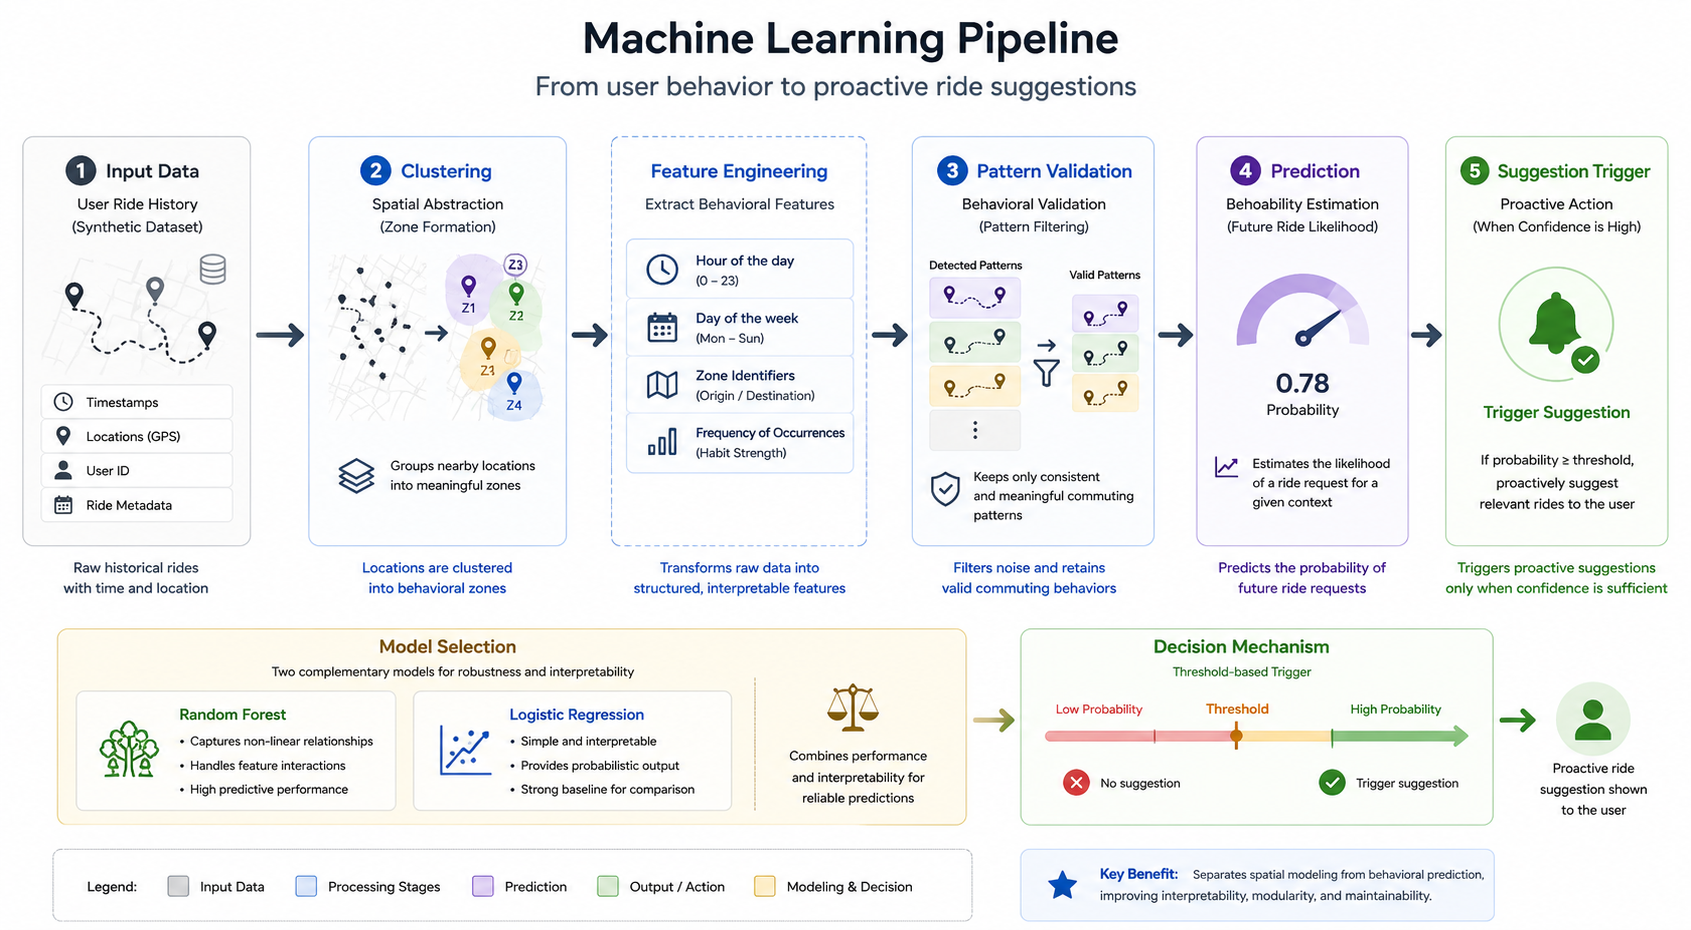
\includegraphics[width=0.95\textwidth]{images/architecture/ml_pipeline.png}
\caption{Machine Learning Pipeline}
\end{figure}
The pipeline is organized into three stages, each addressing a specific aspect of the problem:

\begin{itemize}
    \item \textbf{Clustering Stage}: groups raw trip data into candidate commuting patterns.
    \item \textbf{Pattern Validation Stage}: filters noise and retains stable, recurring patterns.
    \item \textbf{Prediction Stage}: estimates the probability of a user performing a trip at a given time.
\end{itemize}

The pipeline organization reflects a deliberate design choice: separating deterministic structure extraction from probabilistic prediction.

In practice, the platform first identifies consistent behavioral patterns before attempting to predict their occurrence. This prevents the prediction model from being influenced by irregular or isolated observations, which could otherwise degrade performance.

By isolating these stages, the pipeline guarantees that only validated and meaningful patterns are passed to the prediction model, improving both stability and reliability.

This architecture offers several advantages:

\begin{itemize}
    \item improved interpretability of each stage,
    \item reduced model complexity,
    \item easier debugging and validation of intermediate results,
    \item clearer separation between data preparation and decision-making logic.
\end{itemize}

% ------------------------
\subsection{Feature Engineering and Representation}

The effectiveness of the proposed approach depends largely on the design of features that capture both temporal and spatial aspects of user behavior.

The selected features include:

\begin{itemize}
    \item Hour of the day — models daily temporal cycles.
    \item Day of the week — captures weekday versus weekend behavior.
    \item Zone identifiers — represent spatial clustering of locations.
    \item Frequency of occurrence — quantifies the regularity of observed patterns.
\end{itemize}

These features are intentionally simple and interpretable, while remaining directly aligned with the characteristics of commuting behavior.

In addition, this representation avoids unnecessary dimensionality, allowing the model to focus on the most informative signals without introducing redundant or noisy variables.

Unlike high-dimensional feature spaces, this approach keeps the model transparent and easier to analyze, which is particularly important in an academic and system design context~\cite{mitchell1997machine}.

% ------------------------
\subsection{Model Selection and Trade-offs}

Two models are employed:

\begin{itemize}
    \item \textbf{Random Forest}: chosen for its ability to capture non-linear relationships and handle feature interactions with minimal preprocessing~\cite{breiman2001random}.
    \item \textbf{Logistic Regression}: used as a baseline due to its simplicity and interpretability.
\end{itemize}

The use of both models reflects a trade-off between predictive performance and interpretability.

Random Forest generally provides stronger predictive capability when user behavior deviates from simple linear trends, while Logistic Regression offers clearer insight into how individual features influence predictions.

Using both models also enables comparative evaluation, helping to verify that improvements in performance do not come at the expense of explainability.

This dual-model approach ensures that the system remains both effective and transparent, which is essential for validation and future refinement.

% ------------------------
\subsection{Prediction Strategy and Decision Threshold}

The model outputs a probability score representing the likelihood of a commute occurring under given conditions.

A threshold-based mechanism is applied to convert this probability into actionable decisions. Only predictions exceeding a predefined threshold are presented to the user, reducing the risk of irrelevant or excessive suggestions.

This design highlights an important system-level trade-off: prediction accuracy must be balanced with user trust and interface clarity. Over-predicting may reduce confidence in the system, while under-predicting may limit its usefulness.

In practice, the threshold acts as a tunable parameter that can be adjusted based on user feedback or deployment context, allowing the system to adapt its level of proactivity.

The threshold value is selected empirically to balance precision and recall. A higher threshold improves precision but may omit relevant suggestions, while a lower threshold increases coverage at the cost of potential noise. The chosen value reflects a compromise aligned with user experience requirements.

In this context, prioritizing precision is essential to preserve user trust and avoid notification fatigue. The chosen threshold therefore favors relevance over coverage.

While ROC-based analysis could provide additional insight into model discrimination across thresholds, it was not prioritized due to the system's focus on fixed-threshold decision making.

% ------------------------
\subsection{Integration with System Architecture}

This architecture integrates the Machine Learning System as a complementary layer within the overall design.

It operates independently from the core ride management and matching logic, ensuring that:

\begin{itemize}
    \item core functionalities remain unaffected by prediction errors,
    \item the system maintains robustness even if the ML component is disabled,
    \item predictions enhance rather than dictate system behavior.
\end{itemize}

The loose coupling is a deliberate design decision that improves system reliability, simplifies maintenance, and allows the ML component to evolve independently without impacting critical operations.
\subsection{User Interface Integration}

\begin{figure}[H]
\centering
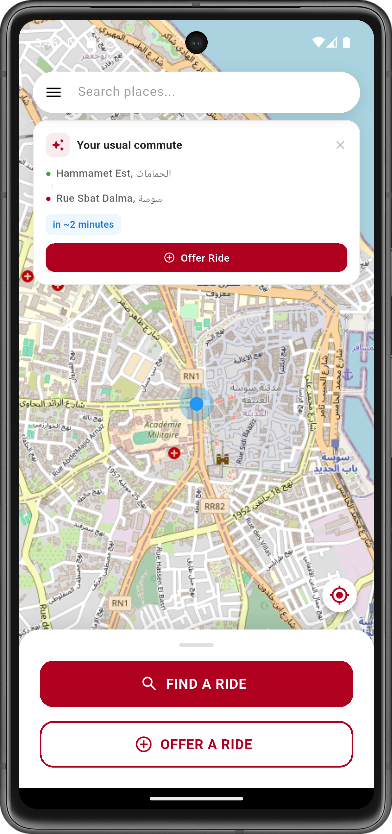
\includegraphics[width=0.3\textwidth]{images/ui/commute_prediction.png}
\caption{Proactive Ride Suggestion}
\end{figure}

Predictions are exposed to the user through a proactive suggestion component integrated into the interface.

This component presents pre-configured ride options derived from predicted behavior, allowing users to respond immediately without manually initiating a search.

The integration bridges the gap between model output and user interaction, translating predictive results into concrete, actionable features.

% ------------------------
\subsection{Sprint Validation and Evaluation}

The Machine Learning System was evaluated using several complementary validation criteria:

\begin{itemize}
    \item \textbf{Pattern Consistency}: verifying that extracted patterns reflect realistic commuting behavior.
    \item \textbf{Prediction Stability}: ensuring that similar inputs lead to consistent outputs.
    \item \textbf{Suggestion Relevance}: assessing whether generated suggestions correspond to expected user needs.
\end{itemize}

Additional controlled scenarios were tested to verify that:

\begin{itemize}
    \item predictions are not generated for irregular or noisy behavior,
    \item suggestions are triggered only within appropriate temporal windows,
    \item system performance remains stable under repeated evaluations.
\end{itemize}

% ------------------------
\subsubsection{Model Specification}

Two classifiers are trained and evaluated:

\begin{itemize}
    \item \textbf{Random Forest (primary)}: selected for its ability to capture non-linear feature interactions without extensive preprocessing, which is well suited for structured commuting behavior~\cite{breiman2001random}.
    \item \textbf{Logistic Regression (baseline)}: used as a reference model due to its simplicity and interpretability~\cite{mitchell1997machine}.
\end{itemize}

Both models operate on the same low-dimensional feature representation, ensuring a fair comparison of their respective capabilities.

% ------------------------
\subsubsection{Training Setup}

The synthetic dataset contains 4,200 labeled commute instances. A stratified 80/20 split is applied, with 3,360 instances used for training and 840 for testing.

Stratification preserves the class distribution across both sets, ensuring that evaluation results remain representative and unbiased.

% ------------------------
\subsubsection{Hyperparameters}

The Random Forest is configured with the following parameters:

\begin{itemize}
    \item \texttt{n\_estimators = 100} -- number of trees in the ensemble,
    \item \texttt{max\_depth = 12} -- maximum tree depth to limit overfitting,
    \item \texttt{min\_samples\_split = 5} -- minimum number of samples required for a split.
\end{itemize}

Logistic Regression uses L2 regularization with \texttt{C = 1.0}, corresponding to a balanced trade-off between model complexity and generalization.

% ------------------------
\subsubsection{Performance Results}

Table~\ref{tab:ml_performance} reports classifier performance on the held-out test set.

\begin{table}[H]
\centering
\renewcommand{\arraystretch}{1.2}
\begin{tabular}{|l|c|c|}
\hline
\textbf{Metric} & \textbf{Random Forest} & \textbf{Logistic Regression} \\
\hline
Accuracy  & 0.82 & 0.74 \\
\hline
Precision & 0.79 & 0.71 \\
\hline
Recall    & 0.85 & 0.78 \\
\hline
F1-score  & 0.82 & 0.74 \\
\hline
\end{tabular}
\caption{Machine Learning Classifier Performance}
\label{tab:ml_performance}
\end{table}

% ------------------------
\subsubsection{Interpretation}

Random Forest achieves higher performance across all metrics, indicating that the relationship between temporal, spatial, and frequency features is not purely linear.

The F1-score of 0.82 reflects a balanced trade-off between precision and recall, which is particularly important in a proactive system where both false positives (irrelevant suggestions) and false negatives (missed opportunities) impact user experience.

These results confirm that the model captures structured behavioral patterns effectively, while also highlighting the limitations introduced by synthetic data when considering real-world deployment.

The observed performance difference also suggests that commuting behavior cannot be fully captured by linear decision boundaries. The results remained consistent across multiple evaluation runs, indicating stable model behavior under similar input conditions.

This consistency reinforces the reliability of the predictive component within the controlled experimental setup. The model shows no signs of severe overfitting, as performance remains consistent between training and test distributions.

In addition, the observed performance reflects a balance between bias and variance. The Random Forest model reduces bias by capturing complex feature interactions, while its ensemble structure limits variance, resulting in more stable predictions compared to simpler linear models.

In addition to standard evaluation metrics such as accuracy, precision, recall, and F1-score, the model performance is further analyzed through the confusion matrix, providing a detailed view of classification errors~\cite{classification}. While advanced evaluation tools such as ROC curves were not explicitly explored, the selected metrics are sufficient to assess model performance within the scope of this study.

The confusion matrix also highlights the trade-off between false positives and false negatives, which is particularly important in controlling the relevance of suggested rides.

However, the evaluation remains limited to controlled synthetic scenarios, and model behavior under highly irregular or sparse data conditions may differ, particularly in real-world deployments.

For example, users with irregular or non-repetitive travel patterns may not be accurately captured by the current model, highlighting the importance of incorporating more diverse real-world data in future iterations.

% ------------------------
\subsection{System Impact}

The integration of the Machine Learning System enhances the overall architecture in several ways:

\begin{itemize}
    \item reduces user effort by eliminating repetitive manual searches,
    \item improves ride discovery through timely and relevant suggestions,
    \item aligns system behavior with individual commuting habits rather than treating all users uniformly.
\end{itemize}

From a broader perspective, the ML layer shifts the platform from a passive request-driven system to one that anticipates user needs. By identifying likely future actions, this component can surface relevant options before explicit input is provided.

Such anticipatory capability increases the likelihood of successful matches and improves overall platform efficiency.

It also establishes a foundation for future extensions, including demand forecasting, adaptive routing, and personalized recommendation strategies.

% ------------------------
\section{Conclusion}

This chapter introduced an intelligent decision layer that extends the proposed approach beyond reactive operation, transforming it into an adaptive and anticipatory system.

The Smart Matching System addressed limitations of traditional ride-sharing approaches by reformulating matching as a trajectory-based optimization problem. By modeling rides as continuous routes and supporting dynamic pickup insertion, this approach improves matching coverage while maintaining route consistency.

In parallel, the Machine Learning System introduces a predictive dimension that anticipates user needs based on recurring behavioral patterns. By generating context-aware suggestions, it reduces user effort and improves interaction efficiency. Importantly, this predictive layer operates independently from the core system, preserving robustness while adding intelligence.

Together, these components form a hybrid architecture in which rule-based mechanisms ensure control and correctness, while probabilistic models provide anticipation and personalization. This separation allows the overall architecture to remain both reliable and flexible.

From a global perspective, the platform evolves through three stages: from a transactional system, to a real-time synchronized environment, and finally to an intelligent system capable of adapting to and anticipating user behavior.

The next chapter focuses on system evaluation and validation, including performance analysis, matching effectiveness, prediction relevance, and future improvements.

Future work may explore integrating real-time user feedback and adaptive learning mechanisms to further refine prediction accuracy and personalization.